%Para slide em "Wide-Screen" usar:
\documentclass[aspectratio=169]{beamer} 

%Para slide "quadrado" usar:
%\documentclass{beamer} 

\usepackage{tikz}
\usepackage[final]{hyperref}
\usepackage{xcolor}
%Elaborado por Mateus Moro Lumertz

\usepackage{multicol}

\author{mateuslumertz}
\definecolor{cor1}{HTML}{499FA4}
\definecolor{cor2}{HTML}{BEC6C3}
\definecolor{cor5}{HTML}{E9BC8B}
\definecolor{cor3}{HTML}{3D4A55}
\definecolor{cor4}{HTML}{008080}
\definecolor{preto}{RGB}{0,0,0}
\definecolor{branco}{RGB}{255,255,255}
% Configuração das Cores
\setbeamercolor{paleta1}{fg=cor1,bg=white}
\setbeamercolor{paleta2}{fg=cor1,bg=white}
\setbeamercolor{estrutura}{fg=cor1,bg=white}
\setbeamercolor{titulo_rodape}{fg=black,bg=white}
\setbeamercolor{data_rodape}{fg=gray,bg=white}
\setbeamercolor{frametitle}{fg=cor1,bg=branco}


% Modelo do rodapé
\defbeamertemplate*{footline}{mytheme}{%
  \leavevmode%
  \hbox{\begin{beamercolorbox}[wd=.5\paperwidth,ht=2.5ex,dp=1.125ex,leftskip=.3cm,rightskip=.3cm]{titulo_rodape}%
    \makebox[2em][l]{{\usebeamerfont{titulo_rodape}\textcolor{cor1}{\insertframenumber}}}%
    {\usebeamercolor{titulo_rodape}\insertshorttitle}
  \end{beamercolorbox}%
  \begin{beamercolorbox}[wd=.2\paperwidth,ht=2.5ex,dp=1.125ex,leftskip=.3cm,rightskip=.3cm]{data_rodape}%
    \usebeamerfont{data_rodape}\insertshortdate%
  \end{beamercolorbox}%
  \begin{beamercolorbox}[wd=.3\paperwidth,ht=2.5ex,dp=1.125ex,leftskip=.3cm,rightskip=.3cm,right]{titulo_rodape}%
    
\includegraphics[width=.1\paperwidth,height=7ex,keepaspectratio]{images/logo.png}\hspace*{2em}%
  \end{beamercolorbox}}%
  \vskip0pt%
  
    \begin{tikzpicture}[remember picture,overlay]
  
    \filldraw[cor2]
    ([xshift=-12cm,yshift=7.5cm]current page.south east)--
    ([xshift=-16cm,yshift=7.5cm]current page.south east)--
    ([xshift=-16cm,yshift=7.62cm]current page.south east)--
    ([xshift=-12cm,yshift=7.62cm]current page.south east)-- cycle
    ;
    \filldraw[cor3]
    ([xshift=-8cm,yshift=7.5cm]current page.south east)--
    ([xshift=-12cm,yshift=7.5cm]current page.south east)--
    ([xshift=-12cm,yshift=7.62cm]current page.south east)--
    ([xshift=-8cm,yshift=7.62cm]current page.south east)-- cycle
    ;
    \filldraw[cor4]
    ([xshift=-4cm,yshift=7.5cm]current page.south east)--
    ([xshift=-8cm,yshift=7.5cm]current page.south east)--
    ([xshift=-8cm,yshift=7.62cm]current page.south east)--
    ([xshift=-4cm,yshift=7.62cm]current page.south east)-- cycle
    ;
    \filldraw[cor5]
    ([xshift=-0cm,yshift=7.5cm]current page.south east)--
    ([xshift=-4cm,yshift=7.5cm]current page.south east)--
    ([xshift=-4cm,yshift=7.62cm]current page.south east)--
    ([xshift=-0cm,yshift=7.62cm]current page.south east)-- cycle
    ;

  \end{tikzpicture}
  
}

% Slide de Título
\defbeamertemplate*{title page}{mytheme}[1][]
{%
  \begin{tikzpicture}[remember picture,overlay]
    \filldraw[cor1]
    (current page.north west) --
    ([yshift=-12cm]current page.north west) --
    ([xshift=-4cm,yshift=-12cm]current page.north east) {[rounded corners=15pt]--
    ([xshift=-4cm,yshift=3cm]current page.south east)} --
    ([yshift=3cm]current page.south west) --
    (current page.south west) --
    (current page.south east) --
    (current page.north east) -- cycle
    ;
  \filldraw[branco]
    (current page.north west) --
    ([yshift=-2.15cm]current page.north west) --
    ([xshift=-3cm,yshift=-2.15cm]current page.north east) {[rounded corners=15pt]--
    ([xshift=-3cm,yshift=3cm]current page.south east)} --
    ([yshift=3cm]current page.south west) --
    (current page.south west) --
    (current page.south east) --
    (current page.north east) -- cycle
    ;
    \filldraw[cor2]
    ([xshift=-0.25cm,yshift=3cm]current page.south east)--
    ([xshift=-2.75cm,yshift=3cm]current page.south east)--
    ([xshift=-2.75cm,yshift=3.85cm]current page.south east)--
    ([xshift=-0.25cm,yshift=3.85cm]current page.south east)-- cycle
    ;
    \filldraw[cor3]
    ([xshift=-0.25cm,yshift=4cm]current page.south east)--
    ([xshift=-2.75cm,yshift=4cm]current page.south east)--
    ([xshift=-2.75cm,yshift=4.85cm]current page.south east)--
    ([xshift=-0.25cm,yshift=4.85cm]current page.south east)-- cycle
    ;
    \filldraw[cor4]
    ([xshift=-0.25cm,yshift=5cm]current page.south east)--
    ([xshift=-2.75cm,yshift=5cm]current page.south east)--
    ([xshift=-2.75cm,yshift=5.85cm]current page.south east)--
    ([xshift=-0.25cm,yshift=5.85cm]current page.south east)-- cycle
    ;
    \filldraw[cor5]
    ([xshift=-0.25cm,yshift=6cm]current page.south east)--
    ([xshift=-2.75cm,yshift=6cm]current page.south east)--
    ([xshift=-2.75cm,yshift=6.85cm]current page.south east)--
    ([xshift=-0.25cm,yshift=6.85cm]current page.south east)-- cycle
    ;
  \node[text=branco,anchor=south west,font=\sffamily\LARGE,text width=.68\paperwidth] 
  at ([xshift=10pt,yshift=-0.5cm]current page.west)
  (title)
  {\raggedright\inserttitle};  
  
  \node[text=cor1,anchor=south west,font=\sffamily\small,text width=.75\paperwidth] 
  at ([xshift=10pt,yshift=3.6cm]current page.west)
  (title)
  {\raggedright Robotics and Computter Vision\, Reinforcement Learning
};  
  
  
 % \node[anchor=west]
 %at ([xshift=10.1cm,yshift=8.5cm]current page.south west)
 % {
\includegraphics[height=1.5cm]{imagens/logo.png}};
  
  \node[anchor=east]
  at ([xshift=-0.15cm,yshift=-1cm]current page.north east)
  {
\includegraphics[width=2.5cm]{images/logo.png}};
  
  \node[text=preto,font=\small\sffamily,anchor=south west]
  at ([xshift=30pt,yshift=0.5cm]current page.south west)
  (date)
  {\insertdate};
  \node[text=preto,font=\small\sffamily,anchor=south west]
  at ([yshift=30pt]date.north west)
  (author)
  {\textbf{Presented by:} Walid Shaker - Siba Issa};
  
  \node[text=preto,font=\small\sffamily,anchor=south west]
  at ([yshift=15pt]date.north west)
  (supervisor)
  {\textbf{Supervised by:} Prof. S. M. Ahsan Kazmi - TA: Mohamed Almadfaa
};

  \end{tikzpicture}%
}

% remove navigation symbols
\setbeamertemplate{navigation symbols}{}



% definition of the itemize templates
\setbeamertemplate{itemize item}[circle]
\setbeamercolor{itemize item}{fg=cor3,bg=white}
\setbeamercolor{itemize subitem}{fg=cor4,bg=white}
\setbeamercolor{itemize subsubitem}{fg=cor2,bg=white}



\title[TSC Adaptation using Deep Q-Learning]{Traffic Signal Control Adaptation using Deep
Q-Learning with Experience Replay
}
%Fusion of Data from Lidar and Camera in Self Driving Cars
\date{November 20, 2022}
\begin{document}
\begin{frame}[plain]
\maketitle
\end{frame}




%%%%%%%%%%%%%%%%%%%%%%%%%%%%%%%%%
% Slide 2 (Presentation Outline)
\begin{frame}
\frametitle{Presentation Outline}

\begin{itemize}
  \item Introduction
  \item  Literature Review
  \item System Modeling and Problem Formalization
  \item Deep Q-Learning Algorithm
  \item Simulation Settings
  \item Simulation Results
  \item Conclusion
\end{itemize}

\end{frame}
%%%%%%%%%%%%%%%%%%%%%%%%%%%%%%%%%
%%%%%%%%%%%%%%%%%%%%%%%%%%%%%%%%%
%%%%%%%%%%%%%%%%%%%%%%%%%%%%%%%%%
%%%%%%%%%%%%%%%%%%%%%%%%%%%%%%%%%
% Slide 2 (Introduction)
\begin{frame}
\frametitle{Introduction}
\begin{itemize}
  \item {\color{cor1}\textbf{Introduction}}
  \item  Literature Review
  \item System Modeling and Problem Formalization
  \item Deep Q-Learning Algorithm
  \item Simulation Settings
  \item Simulation Results
  \item Conclusion
\end{itemize}

\end{frame}
%%%%%%%%%%%%%%%%%%%%%%%%%%%%%%%%%
% Slide 3 (Introduction)
\begin{frame}
\frametitle{Introduction}
\framesubtitle{}

Traffic congestion has always been a major issue that
disrupts our lives, make us late for work, and harms the
environment due to the amount of fuel consumed. Despite the
massive studies conducted on these issues, traffic monitoring,
control, and congestion alleviation approaches continue to be
popular research topics.

\end{frame}
%%%%%%%%%%%%%%%%%%%%%%%%%%%%%%%%%
%%%%%%%%%%%%%%%%%%%%%%%%%%%%%%%%%
%%%%%%%%%%%%%%%%%%%%%%%%%%%%%%%%%
%%%%%%%%%%%%%%%%%%%%%%%%%%%%%%%%%
% Slide 4 (Literature Review)
\begin{frame}
\frametitle{Literature Review}
\begin{itemize}
  \item  Introduction
  \item {\color{cor1}\textbf{Literature Review}}
  \item System Modeling and Problem Formalization
  \item Deep Q-Learning Algorithm
  \item Simulation Settings
  \item Simulation Results
  \item Conclusion
\end{itemize}

\end{frame}
%%%%%%%%%%%%%%%%%%%%%%%%%%%%%%%%%
% Slide 3 (Literature Review)
\begin{frame}
\frametitle{Literature Review}
\framesubtitle{}

When we searched the literature for solutions to traffic
congestion issues, we found two fundamental classifications:
\begin{enumerate}
    \item Based on the features considered for traffic light control (human-crafted features \& machine-crafted features)
    \item The used approach (fixed-time \& adaptive))
\end{enumerate}
\end{frame}
%%%%%%%%%%%%%%%%%%%%%%%%%%%%%%%%%
%%%%%%%%%%%%%%%%%%%%%%%%%%%%%%%%%
%%%%%%%%%%%%%%%%%%%%%%%%%%%%%%%%%
%%%%%%%%%%%%%%%%%%%%%%%%%%%%%%%%%
%%%%%%%%%%%%%%%%%%%%%%%%%%%%%%%%%
% Slide  (System Modeling and Problem Formalization)
\begin{frame}
\frametitle{System Modeling and Problem Formalization}
\begin{itemize}
  \item  Introduction
  \item Literature Review
  \item {\color{cor1}\textbf{System Modeling and Problem Formalization}}
  \item Deep Q-Learning Algorithm
  \item Simulation Settings
  \item Simulation Results
  \item Conclusion
\end{itemize}

\end{frame}
%%%%%%%%%%%%%%%%%%%%%%%%%%%%%%%%%
% Slide 3 (System Modeling and Problem Formalization)
\begin{frame}
\frametitle{System Modeling and Problem Formalization}
\framesubtitle{}
\vspace{1cm}

\begin{minipage}{0.3\textwidth}
\begin{itemize}
    \item Environment
    \item Traffic light system (agent)
\end{itemize}
\end{minipage}%
\hfill
\begin{minipage}{0.7\textwidth}
\begin{figure}
    \centering
    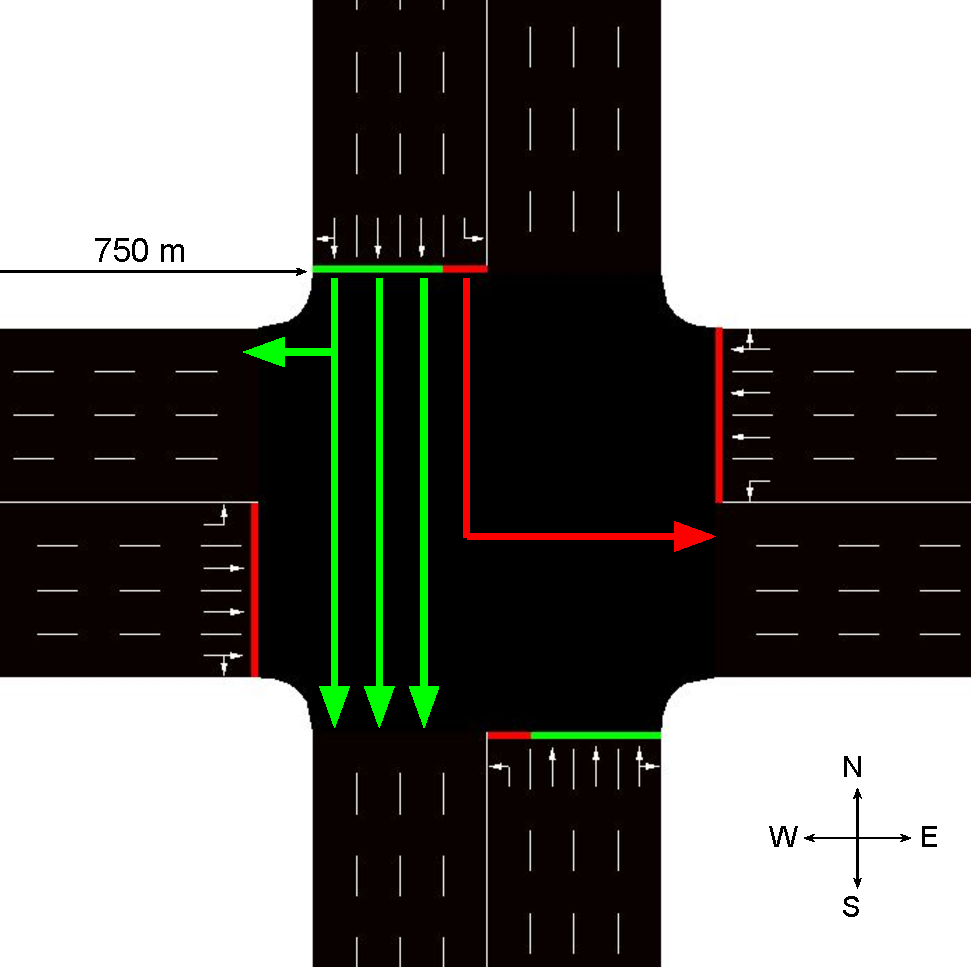
\includegraphics[width=0.6\linewidth]{images/Intersection.pdf}
\end{figure}
\end{minipage}
\end{frame}

%%%%%%%%%%%%%%%%%%%%%%%%%%%%%%%%%
\begin{frame}
\frametitle{System Modeling and Problem Formalization}
\framesubtitle{}
We can define the addressed problem as follows: given a state of intersection, and in order to maximize the intersection’s traffic
efficiency, which traffic light stage the agent has to select
from a fixed predefined set of actions.
\end{frame}
%%%%%%%%%%%%%%%%%%%%%%%%%%%%%%%%%
% Slide 3 (System Modeling and Problem Formalization)
\begin{frame}
\frametitle{System Modeling and Problem Formalization}
\framesubtitle{}
\vspace{1cm}

\begin{minipage}{0.3\textwidth}
\begin{itemize}
    \item sumo step
    \item agentstep
    \item $S_{t}, A_{t}, R_{t}, S_{t+1}$
\end{itemize}
\end{minipage}%
\hfill
\begin{minipage}{0.7\textwidth}
\begin{figure}
    \centering
    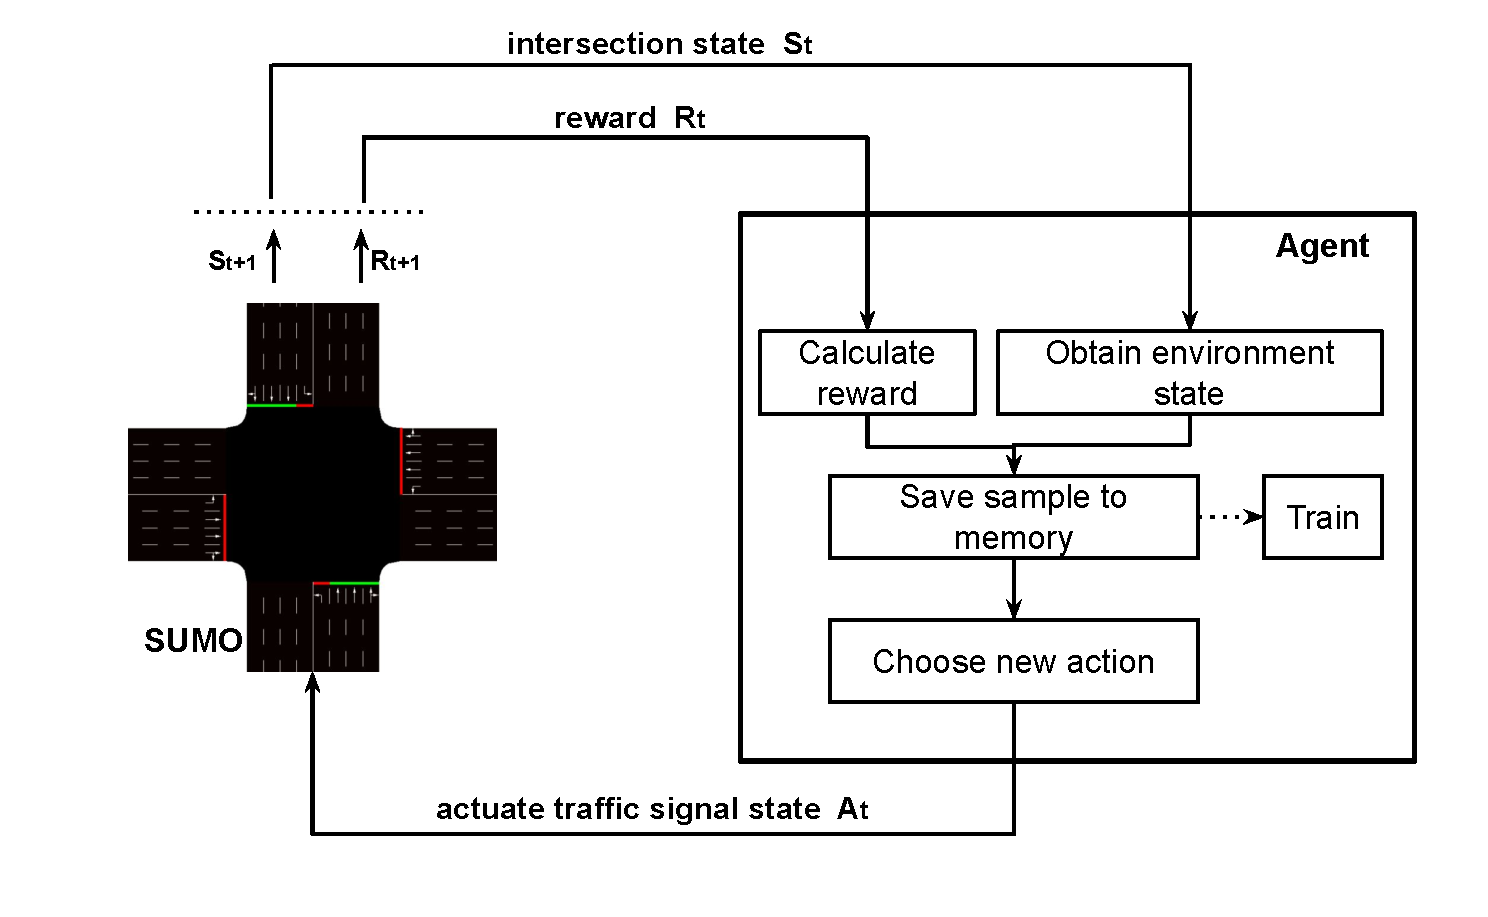
\includegraphics[width=1\linewidth]{images/RL_TSC_Scheme.pdf}
\end{figure}
\end{minipage}
\end{frame}
%%%%%%%%%%%%%%%%%%%%%%%%%%%%%%%%%
% Slide 3 (System Modeling and Problem Formalization)
\begin{frame}
\frametitle{System Modeling and Problem Formalization}
\framesubtitle{Environment State}
\vspace{1cm}

\begin{minipage}{0.3\textwidth}
\begin{itemize}
    \item Road discretization (1,0)
    \item 20 cells per road, 80 cells in total
\end{itemize}
\end{minipage}%
\hfill
\begin{minipage}{0.7\textwidth}
\begin{figure}
    \centering
    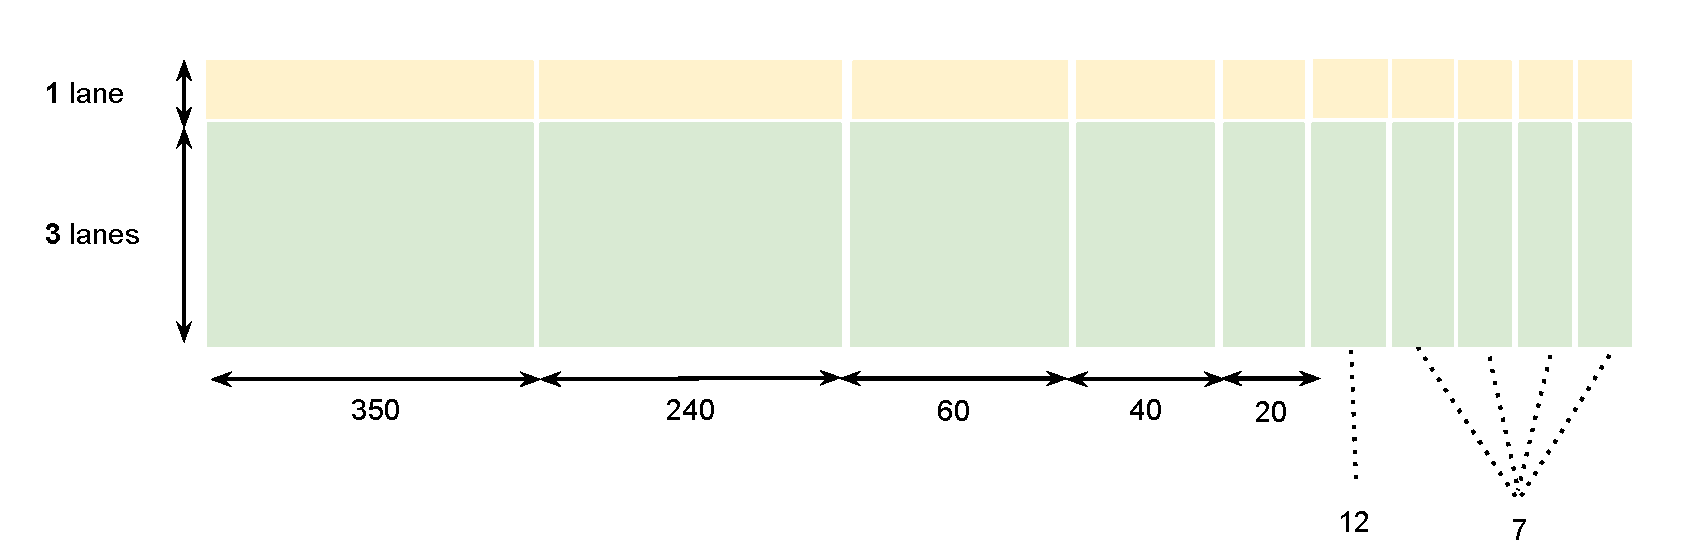
\includegraphics[width=1\linewidth]{images/State cells length.pdf}
\end{figure}
\end{minipage}
\end{frame}
%%%%%%%%%%%%%%%%%%%%%%%%%%%%%%%%%
% Slide 3 (System Modeling and Problem Formalization)
\begin{frame}
\frametitle{System Modeling and Problem Formalization}
\framesubtitle{Agent Action Set}
\vspace{1cm}
\begin{minipage}{0.1\textwidth}
    $A = \{NS, EW, NSL, EWL\}$
\end{minipage}%
\vfill
\begin{minipage}{1\textwidth}
\begin{figure}
    \centering
    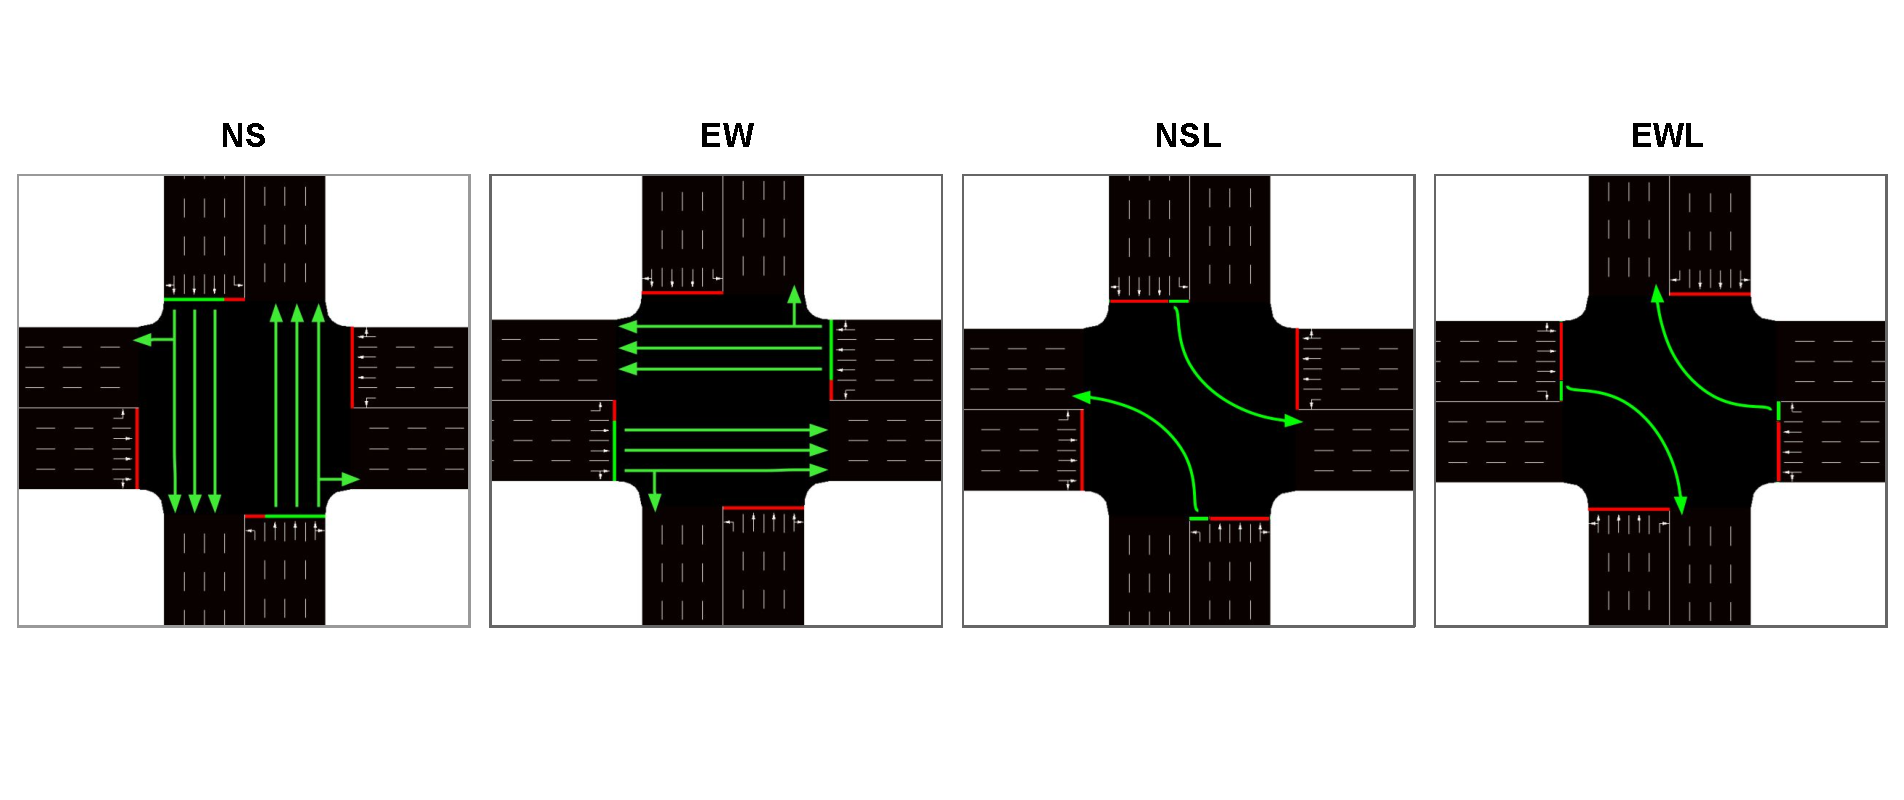
\includegraphics[width=1\linewidth]{images/Possible actions.pdf}
\end{figure}
\end{minipage}
\end{frame}

%%%%%%%%%%%%%%%%%%%%%%%%%%%%%%%%%
% Slide 3 (System Modeling and Problem Formalization)
\begin{frame}
\frametitle{System Modeling and Problem Formalization}
\framesubtitle{Agent Action Set}

\begin{figure}
    \centering
    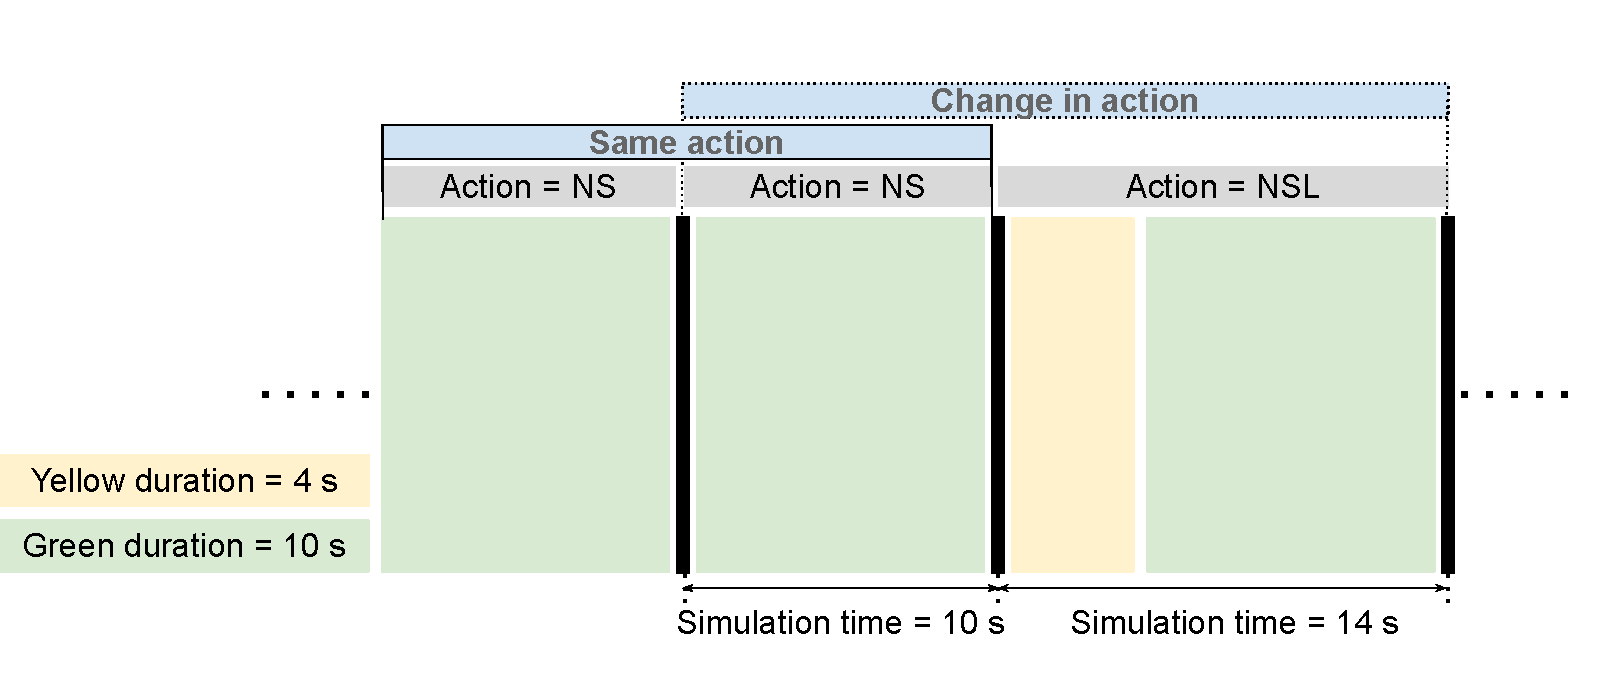
\includegraphics[width=0.8\linewidth]{images/Simulation steps.pdf}
    \caption{Possible simulation time of chosen actions.}
\end{figure}

\end{frame}
%%%%%%%%%%%%%%%%%%%%%%%%%%%%%%%%%
% Slide 3 (System Modeling and Problem Formalization)
\begin{frame}
\frametitle{System Modeling and Problem Formalization}
\framesubtitle{Reward Function}
In our problem, our goal is to reduce vehicle waiting time at traffic lights, but we want to cast it as a maximization problem, so our goal is to increase traffic flow through the intersection over time. \\
\textbf{Literature reward function:}
\begin{equation}
\label{Eq:3}
    r_t= twt_{t-1} - twt_t
\end{equation}
\begin{equation}
\label{Eq:2}
    twt_t= \sum_{veh=1}^{n} {wt_{veh,t}}
\end{equation}


\end{frame}
%%%%%%%%%%%%%%%%%%%%%%%%%%%%%%%%%
% Slide 3 (System Modeling and Problem Formalization)
\begin{frame}
\frametitle{System Modeling and Problem Formalization}
\framesubtitle{Reward Function}
\textbf{Aternative reward function}

\begin{equation}
\label{Eq:5}
    r_t= atwt_{t-1} - atwt_t
\end{equation}
    
\begin{equation}
\label{Eq:4}
    atwt_t= \sum_{veh=1}^{n} {awt_{veh,t}}
\end{equation}
 Where $atwt_t$ represents the accumulated waiting time. By using this reward function we can guarantee that when the vehicle departs but could not cross the intersection, the value of $atwt_t$ does not reset (unlike the value of $twt_t$), avoiding the misleading case associated with the literature reward function when a long queue appears at the intersection.
\end{frame}
%%%%%%%%%%%%%%%%%%%%%%%%%%%%%%%%%
% Slide 3 (System Modeling and Problem Formalization)
\begin{frame}
\frametitle{System Modeling and Problem Formalization}
\framesubtitle{Agent Goal}
The main goal in our case is to increase traffic flow through the intersection by reducing the vehicles waiting time. The agent must choose the appropriate action, which will be in accordance with action policy $\pi^*$. \\
\textbf{Expected cumulative reward: }
\begin{equation}
    \label{Eq:6}
    Q_{\pi}(s,a) = \mathop{\mathbb{E}}\{ R_t+\gamma R_{t+1} + \gamma^2R_{t+2}+...|S_t=s,A_t=a,\pi\}
\end{equation}
\begin{equation*}
    = \mathop{\mathbb{E}}\{\sum_{k=0}^{\infty}\gamma^kR_{t+k}|S_t=s,A_t=a,\pi\}
\end{equation*}
Such an optimal policy $\pi^*$ can be given by
\begin{equation}
    \pi^*= \underset{\pi}{\operatorname{argmax}} Q_\pi(s,a) \quad for \quad all \quad s\in S, a \in A
\end{equation}
\end{frame}

%%%%%%%%%%%%%%%%%%%%%%%%%%%%%%%%%
%%%%%%%%%%%%%%%%%%%%%%%%%%%%%%%%%
%%%%%%%%%%%%%%%%%%%%%%%%%%%%%%%%%
%%%%%%%%%%%%%%%%%%%%%%%%%%%%%%%%%
%%%%%%%%%%%%%%%%%%%%%%%%%%%%%%%%%
% Slide  (Deep Q-Learning Algorithm)
\begin{frame}
\frametitle{Deep Q-Learning Algorithm}
\begin{itemize}
  \item  Introduction
  \item Literature Review
  \item System Modeling and Problem Formalization
  \item {\color{cor1}\textbf{Deep Q-Learning Algorithm}}
  \item Simulation Settings
  \item Simulation Results
  \item Conclusion
\end{itemize}

\end{frame}
%%%%%%%%%%%%%%%%%%%%%%%%%%%%%%%%%
% Slide 3 (System Modeling and Problem Formalization)
\begin{frame}
\frametitle{Deep Q-Learning Algorithm}
\framesubtitle{}

If the optimal Q-values $Q^*(s,a)$ for all pairs of state-action are known, the agent can find the optimal action policy $\pi^*$ by basically picking the action $a$ that results in the optimal Q-values $Q^*(s,a)$ for a state $s$. The optimal Q-values $Q^*(s,a)$ can be calculated from Bellman optimality recursive equation. 

\begin{equation}
\begin{aligned}
     Q^*(s, a)=\mathbb{\mathbb{E}}\{R_t+\gamma \underset{a^{\prime}}{\operatorname{max}}Q^*(S_{t+1}, a^{\prime})| S_t=s, A_t=a\} \\
    \quad for \quad all \quad s\in S, a \in A
\end{aligned}
\end{equation}
\begin{itemize}
    \item large state space
    \item dynamic environment (transition probability ?) 
\end{itemize}
\end{frame}

\begin{frame}
\frametitle{Deep Q-Learning Algorithm}
\framesubtitle{}

Why Q-Learning? model-free reinforcement learning approach where there is no need for these transition probabilities. The action value function $Q\left(s_t, a_t\right)$ of picking action $a_t$ at state $s_t$ is defined as follows.
\begin{equation}
   Q(S_{t},a_{t})= Q(S_{t},a_{t})+\alpha(r_{t+1}+\gamma \cdot \max_{A}Q(s_{t+1},a_{t})-Q(s_{t},a_{t}))
\end{equation}
Another modified version is used to calculate the Q-Learning function as follows.
\begin{equation}
   \label{Eq:10}
   Q(S_{t},a_{t})= r_{t+1}+\gamma \cdot \max_{A}Q^{\prime}(s_{t+1},a_{t+1})
\end{equation}
Due to the large state space, a deep neural network (DNN) is used to approximate the Q-learning function that results in $Q(s, a) \approx Q^*(s, a)$.
\end{frame}

\begin{frame}
\frametitle{Deep Q-Learning Algorithm}
\framesubtitle{Deep Neural Network Architecture}

\begin{figure}
    \centering
    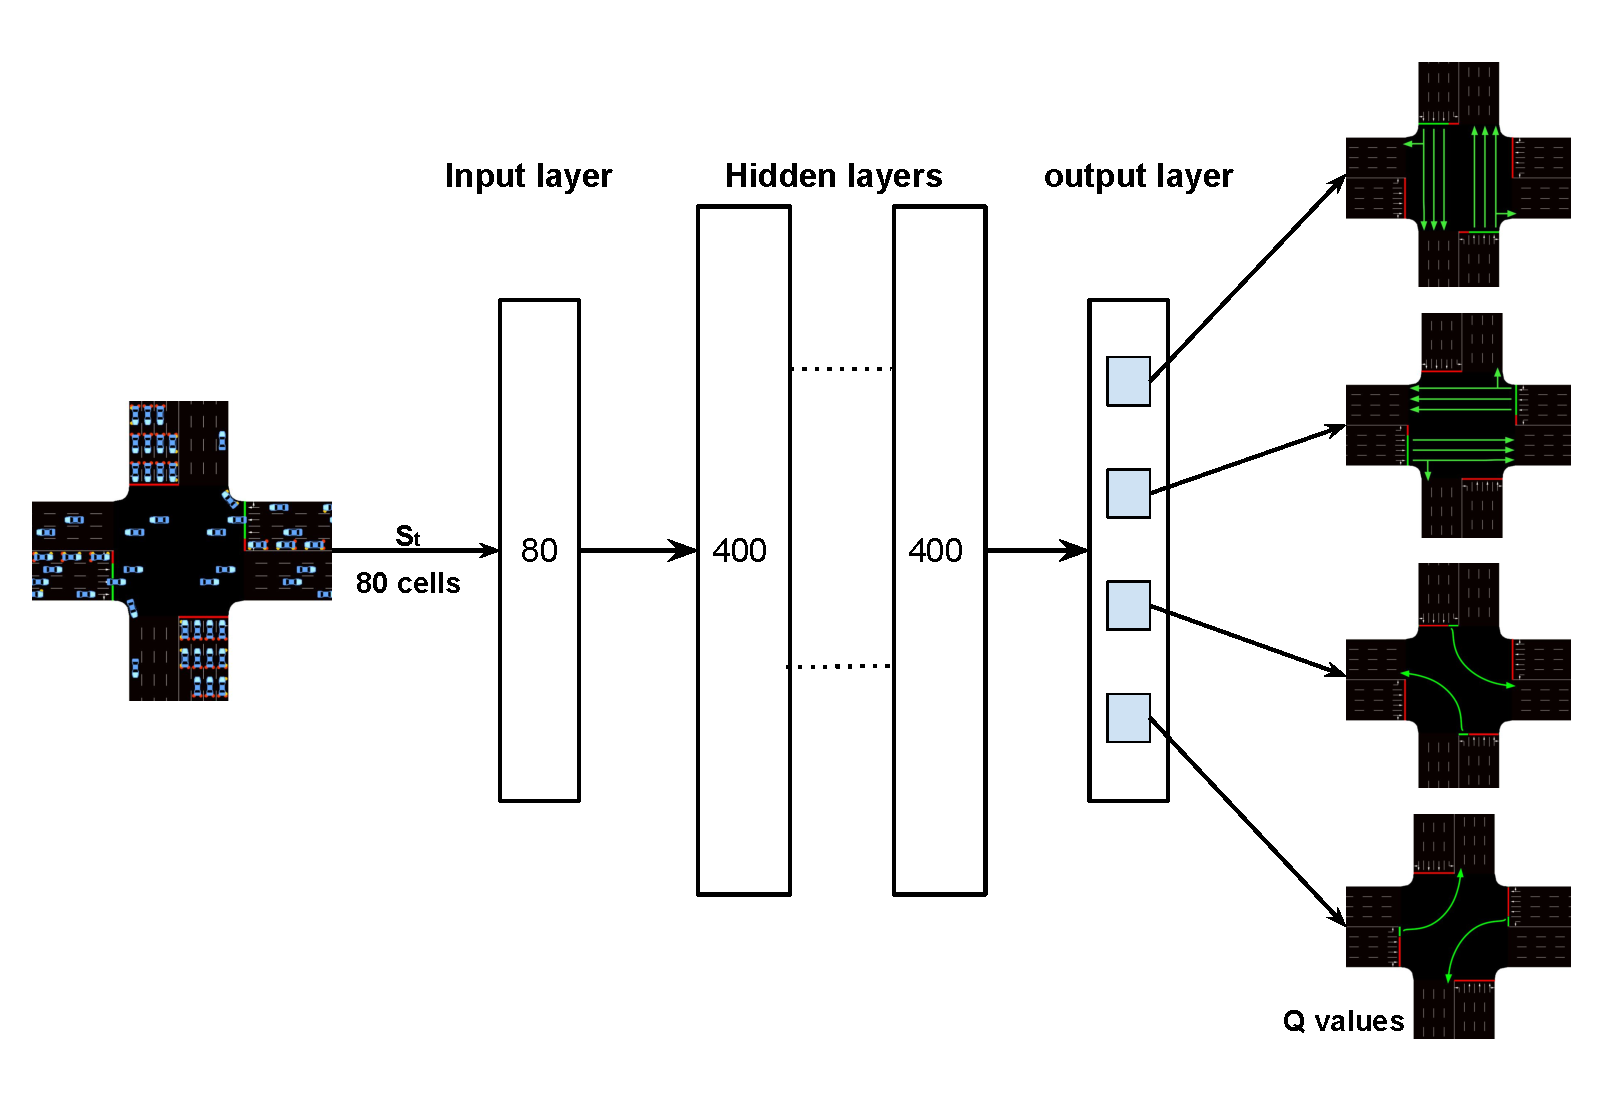
\includegraphics[width=0.62\linewidth]{images/DNN.pdf}
    \caption{Deep neural network architecture.}
\end{figure}

\end{frame}
%%%%%%%%%%%%%%%%%%%%%%%%%%%%%%%%%

\begin{frame}
\frametitle{Deep Q-Learning Algorithm}
\framesubtitle{Experience Replay}
\begin{minipage}{0.4\textwidth}
    \begin{itemize}
        \item Improve model performance 
        \item randomized batch of samples
        \item eliminate correlations
        \item $E_t = \{S_{t}, A_{t}, R_{t+1}, S_{t+1}\}$
        \item $M = \{E_{t}, E_{t+1}, E_{t+2}, \cdots\}$
        \item Memory size = 5000
        \item Batch size = 100
    \end{itemize}


\end{minipage}%
\hfill
\begin{minipage}{0.4\textwidth}
\begin{figure}
    \centering
    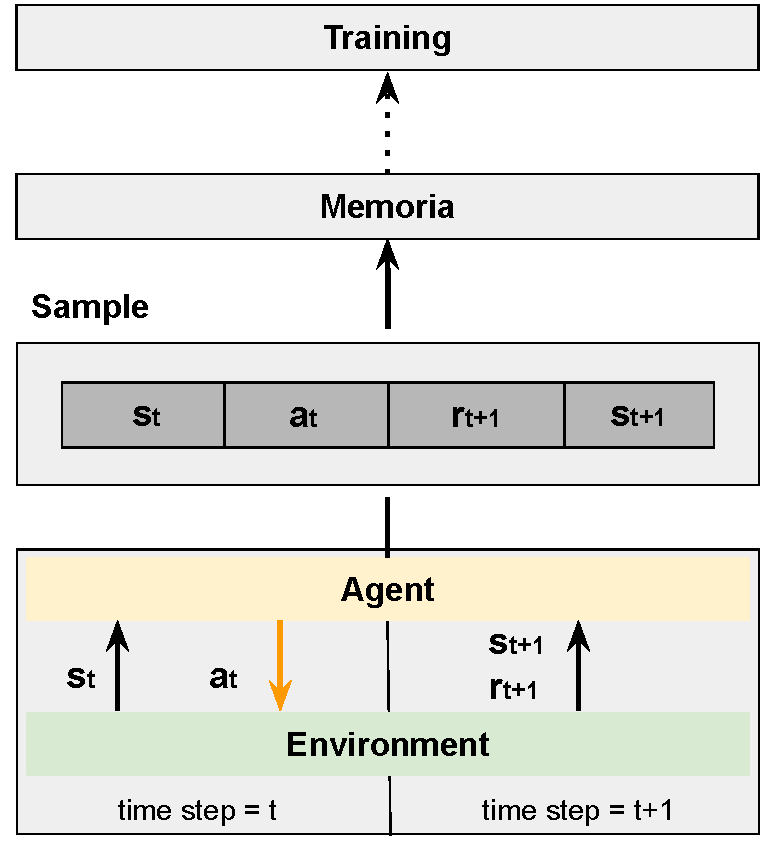
\includegraphics[width=1\linewidth]{images/Data_collection.pdf}
\end{figure}
\end{minipage}
\end{frame}

\begin{frame}
\frametitle{Deep Q-Learning Algorithm}
\framesubtitle{Training Process}
\begin{minipage}{0.4\textwidth}
During the update of $Q(s, a)$, the greedy method is adopted to choose the action that maximizes the predicted action value function $Q^{\prime}(s_{t+1},a_{t+1})$.\\

While acting, the $\epsilon-greedy$ policy, which performs the exploration with probability $\epsilon$ and chooses the exploitation with probability $1-\epsilon$. 

$\epsilon_{n} = 1 - \frac{n}{N}$

\end{minipage}%
\hfill
\begin{minipage}{0.6\textwidth}
\begin{figure}
    \centering
    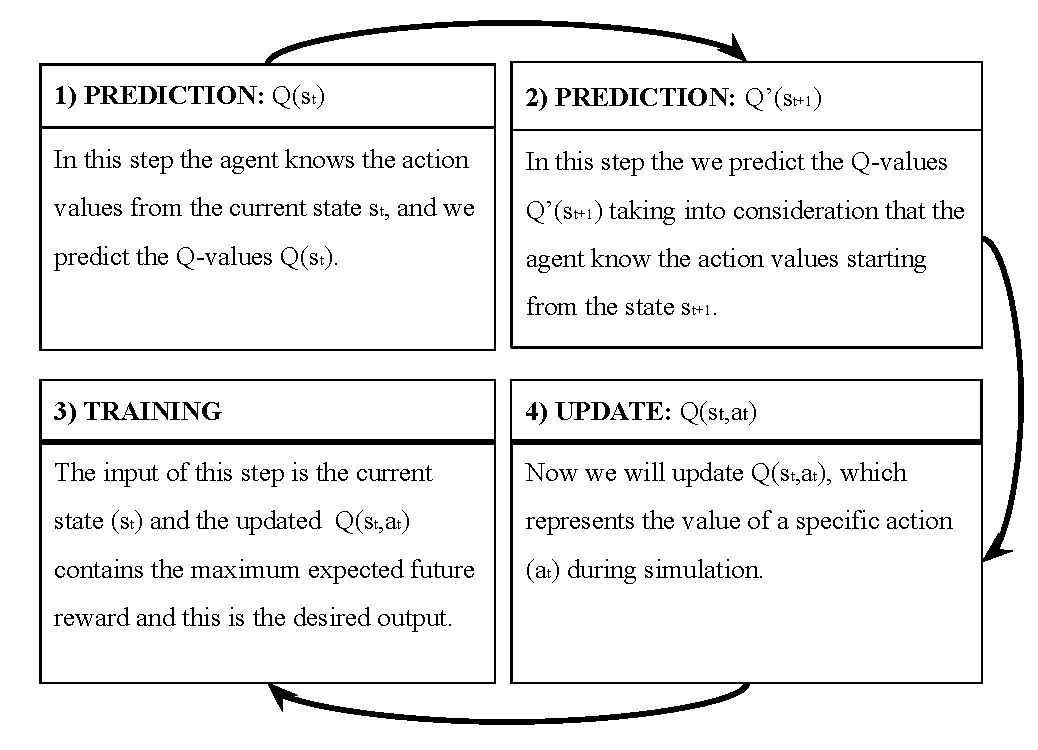
\includegraphics[width=1\linewidth]{images/Training process.pdf}
\end{figure}
\end{minipage}
\end{frame}
%%%%%%%%%%%%%%%%%%%%%%%%%%%%%%%%%

%%%%%%%%%%%%%%%%%%%%%%%%%%%%%%%%%
%%%%%%%%%%%%%%%%%%%%%%%%%%%%%%%%%
%%%%%%%%%%%%%%%%%%%%%%%%%%%%%%%%%
%%%%%%%%%%%%%%%%%%%%%%%%%%%%%%%%%
%%%%%%%%%%%%%%%%%%%%%%%%%%%%%%%%%
% Slide  (Simulation Settings)
\begin{frame}
\frametitle{Simulation Settings}
\begin{itemize}
  \item  Introduction
  \item Literature Review
  \item System Modeling and Problem Formalization
  \item Deep Q-Learning Algorithm
  \item {\color{cor1}\textbf{Simulation Settings}}
  \item Simulation Results
  \item Conclusion
\end{itemize}

\end{frame}
%%%%%%%%%%%%%%%%%%%%%%%%%%%%%%%%%
% Slide 3 (Simulation Settings)
\begin{frame}
\frametitle{Simulation Settings}
\framesubtitle{Training Setup}

\begin{enumerate}
    \item \textbf{Environment:} SUMO simulator provides a time frequency of 1 second per step.
    \item  \textbf{Training Time: } Duration for each episode to 2 hours $2\times60\times60=7200$ steps. 
    \item \textbf{Episode numbers:} 100 episode of 2 hours each, which is more than eight days of continuous traffic.
    \item \textbf{High-graphics laptop}
    \item \textbf{Training time} $3.5$ hours.
\end{enumerate}

\end{frame}
%%%%%%%%%%%%%%%%%%%%%%%%%%%%%%%%%

\begin{frame}
\frametitle{Deep Q-Learning Algorithm}
\framesubtitle{Experience Replay}
\begin{minipage}{0.4\textwidth}
\begin{enumerate}
    \item [-] High traffic scenario: 4000 cars reach the intersection.
    \item [-] Low traffic scenario: 600 cars arrive at the intersection.
    \item [-] North-South (NS) traffic scenario: 2000 cars arriving at the intersection.
    \item [-] East-West (EW) West traffic scenario: 2000 cars arriving at the intersection.
\end{enumerate}

\end{minipage}%
\hfill
\begin{minipage}{0.6\textwidth}
\begin{figure}
    \centering
    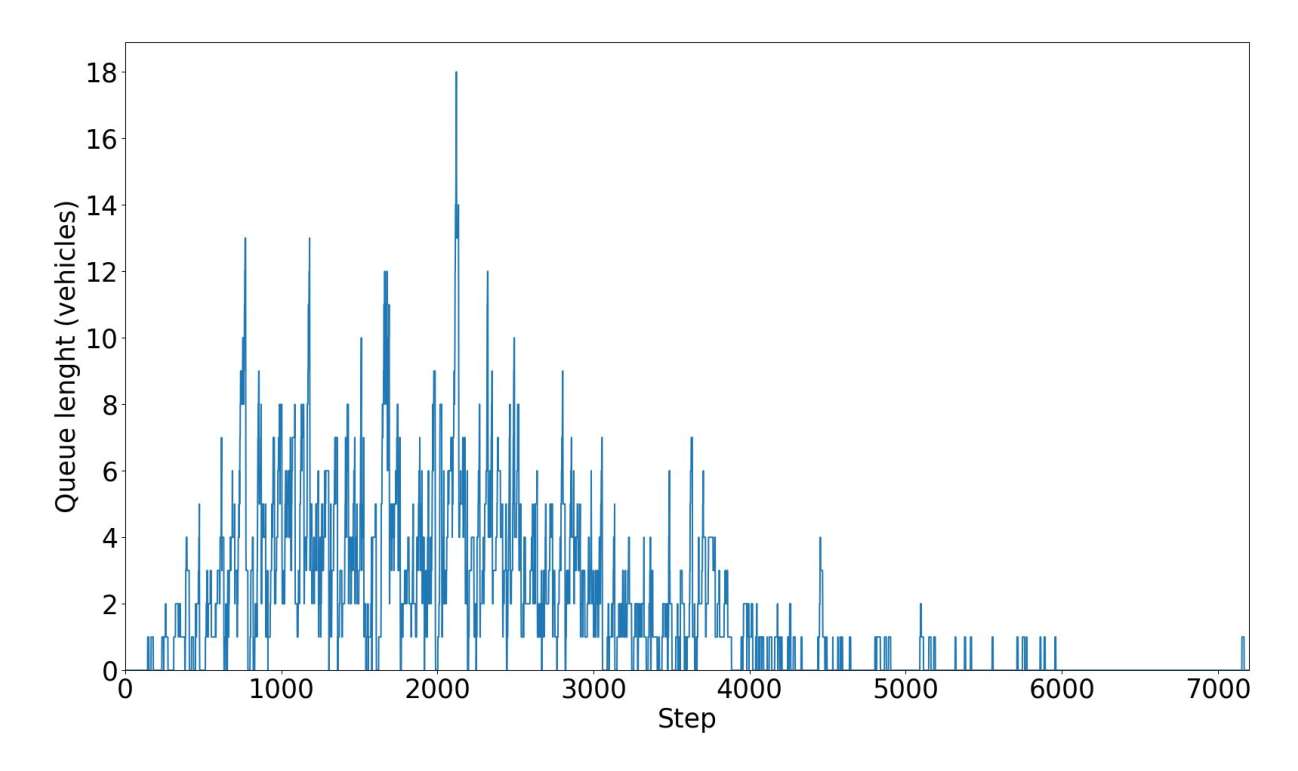
\includegraphics[width=1\linewidth]{images/weibull.pdf} 
\end{figure}
\end{minipage}
\end{frame}
%%%%%%%%%%%%%%%%%%%%%%%%%%%%%%%%%
%%%%%%%%%%%%%%%%%%%%%%%%%%%%%%%%%
%%%%%%%%%%%%%%%%%%%%%%%%%%%%%%%%%
%%%%%%%%%%%%%%%%%%%%%%%%%%%%%%%%%
%%%%%%%%%%%%%%%%%%%%%%%%%%%%%%%%%
% Slide  (Simulation Results)
\begin{frame}
\frametitle{Simulation Results}
\vspace{1cm}
\begin{itemize}
  \item  Introduction
  \item Literature Review
  \item System Modeling and Problem Formalization
  \item Deep Q-Learning Algorithm
  \item Simulation Settings
  \item {\color{cor1}\textbf{Simulation Results}}
  \item Conclusion
\end{itemize}

\end{frame}
%%%%%%%%%%%%%%%%%%%%%%%%%%%%%%%%%
% Slide 3 (Simulation Results)
\begin{frame}
\frametitle{Simulation Results}
\framesubtitle{}
\vspace{1cm}
\begin{minipage}{0.4\textwidth}
The agent performance is examined using the training's reward trend followed by some metrics such as the average queue length (number of vehicles) and the cumulative delay time for all vehicles at the intersection. 

\end{minipage}%
\hfill
\begin{minipage}{0.6\textwidth}
\begin{figure}
    \centering
    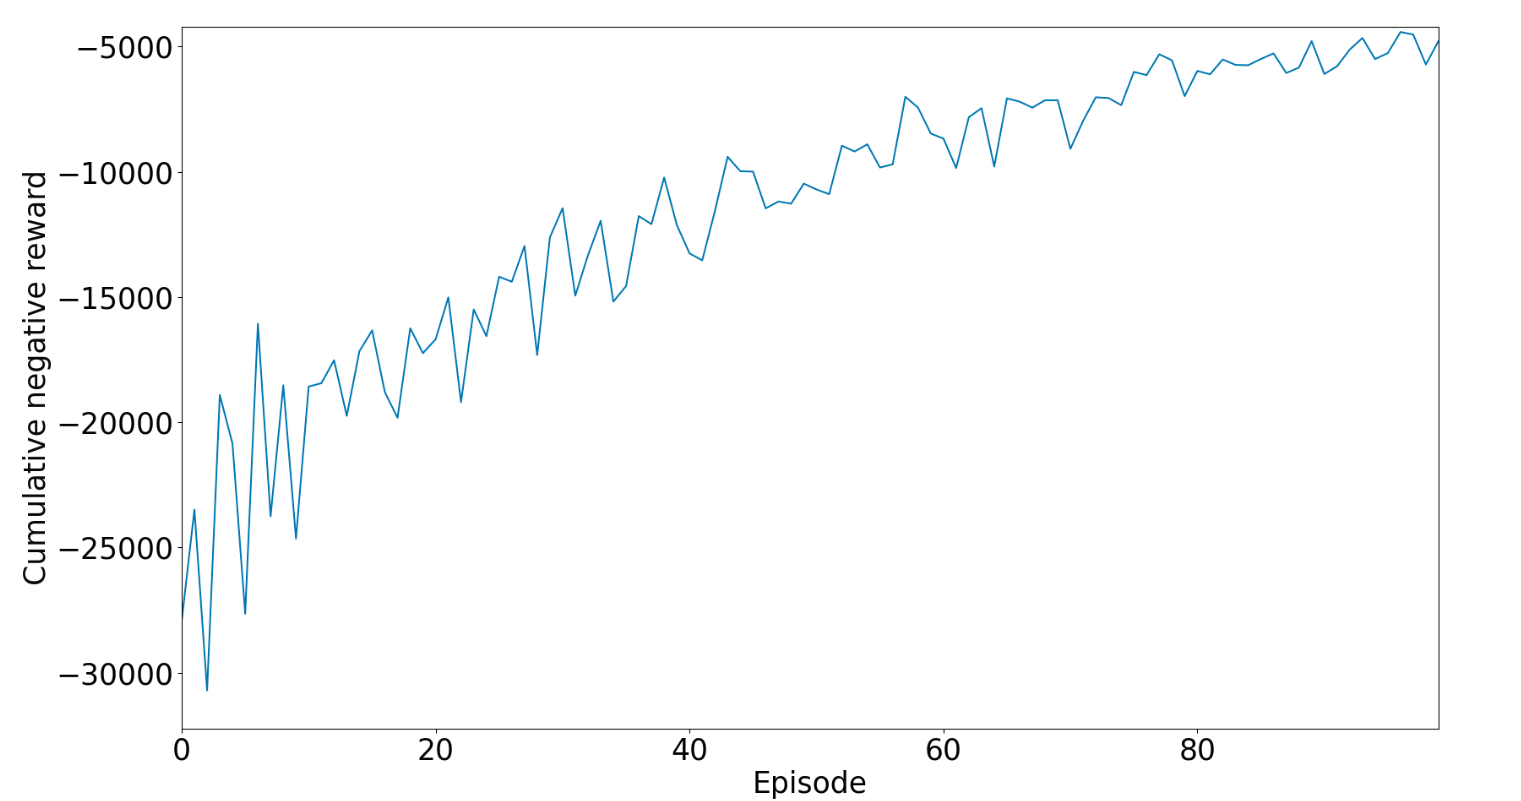
\includegraphics[width=1\linewidth]{images/train_reward.png}
\end{figure}
\end{minipage}
\end{frame}

%%%%%%%%%%%%%%%%%%%%%%%%%%%%%%%%%
% Slide 3 (Simulation Results)
\begin{frame}
\frametitle{Simulation Results}
\framesubtitle{}
\vspace{1cm}
\begin{minipage}{0.4\textwidth}
The total accumulative waiting time (delay) was measured during the training using the alternative reward function which accumulates each waiting time for the vehicle until it passes the intersection.

\end{minipage}%
\hfill
\begin{minipage}{0.6\textwidth}
\begin{figure}
    \centering
    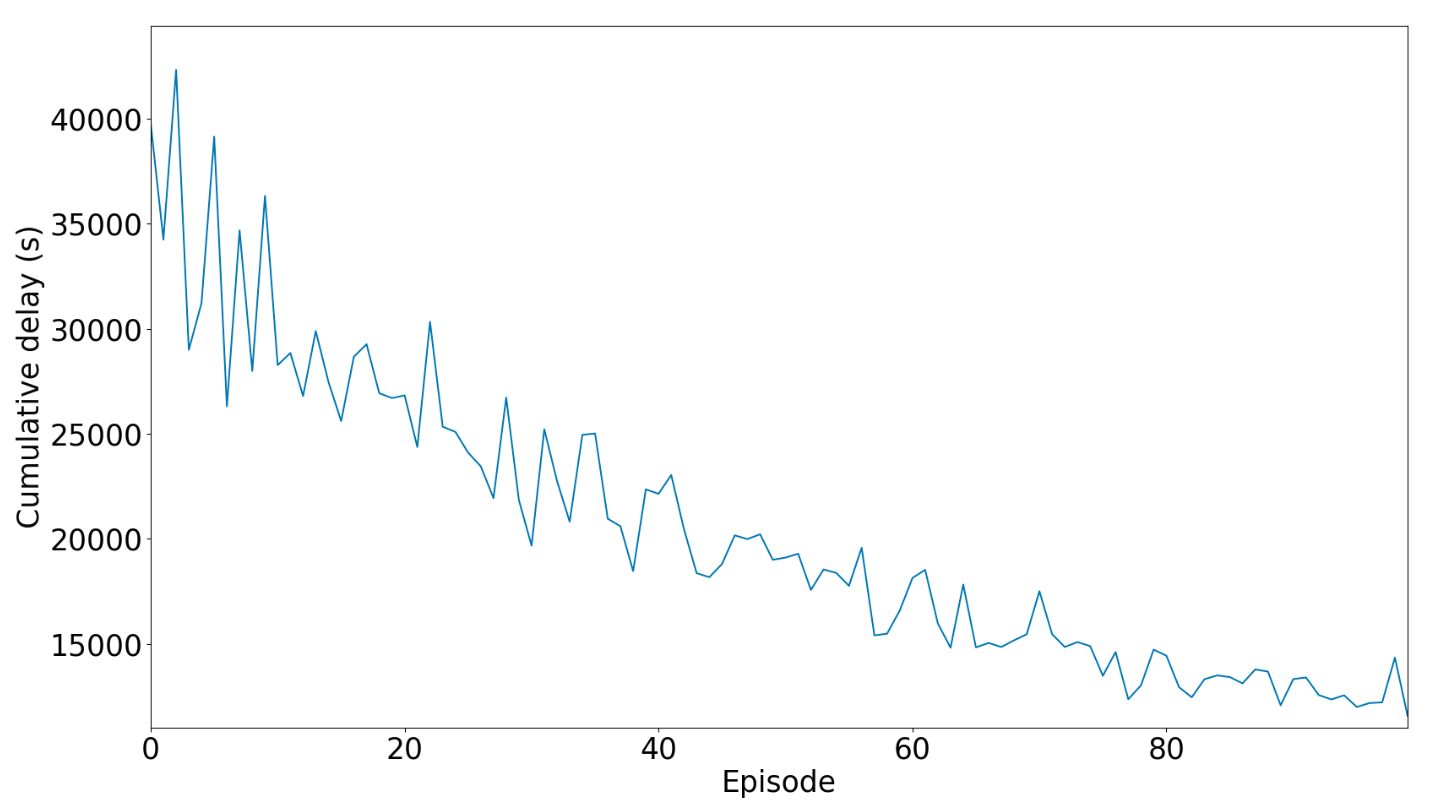
\includegraphics[width=1\linewidth]{images/train_delay.png}
\end{figure}
\end{minipage}
\end{frame}
%%%%%%%%%%%%%%%%%%%%%%%%%%%%%%%%%
% Slide 3 (Simulation Results)
\begin{frame}
\frametitle{Simulation Results}
\framesubtitle{}
\vspace{1cm}
\begin{minipage}{0.4\textwidth}
The corresponding metric for the cumulative waiting time is the queue length, which indicates the average number of cars queued per step in each episode.

\end{minipage}%
\hfill
\begin{minipage}{0.6\textwidth}
\begin{figure}
    \centering
    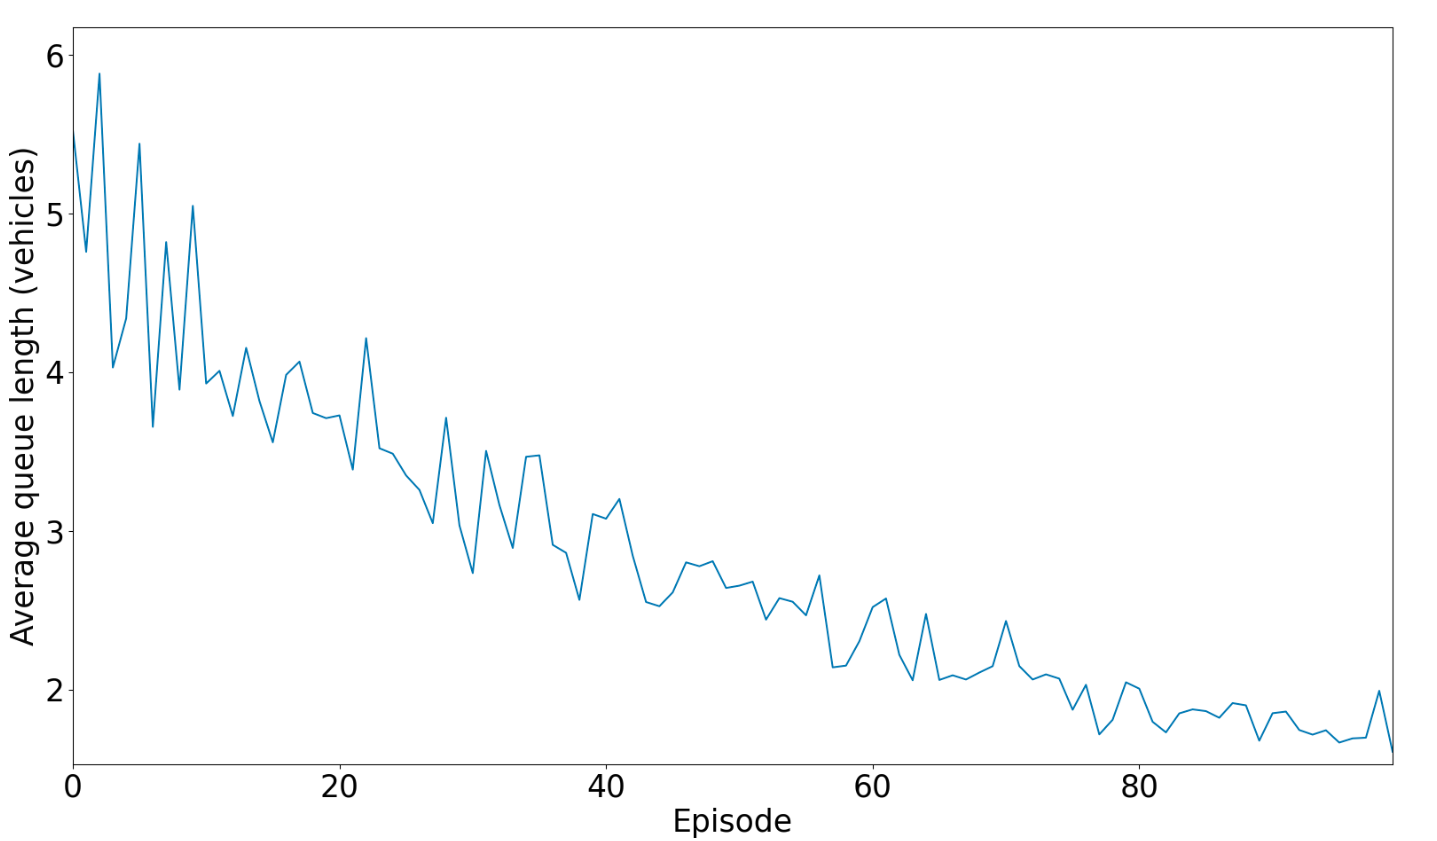
\includegraphics[width=1\linewidth]{images/train_queue.png}
\end{figure}
\end{minipage}
\end{frame}
%%%%%%%%%%%%%%%%%%%%%%%%%%%%%%%%%
% Slide 3 (Simulation Results)
\begin{frame}
\frametitle{Simulation Results}
\framesubtitle{}
\vspace{1cm}
\begin{minipage}{0.4\textwidth}
Model testing is performed and the associated reward to
the actions taken at the agentstep is recorded.\\

\href{https://github.com/Reinforcement-Learning-F22/Traffic-Signal-Control-using-Deep-Q-Learning}{SUMO results} 

\end{minipage}%
\hfill
\begin{minipage}{0.6\textwidth}
\begin{figure}
    \centering
    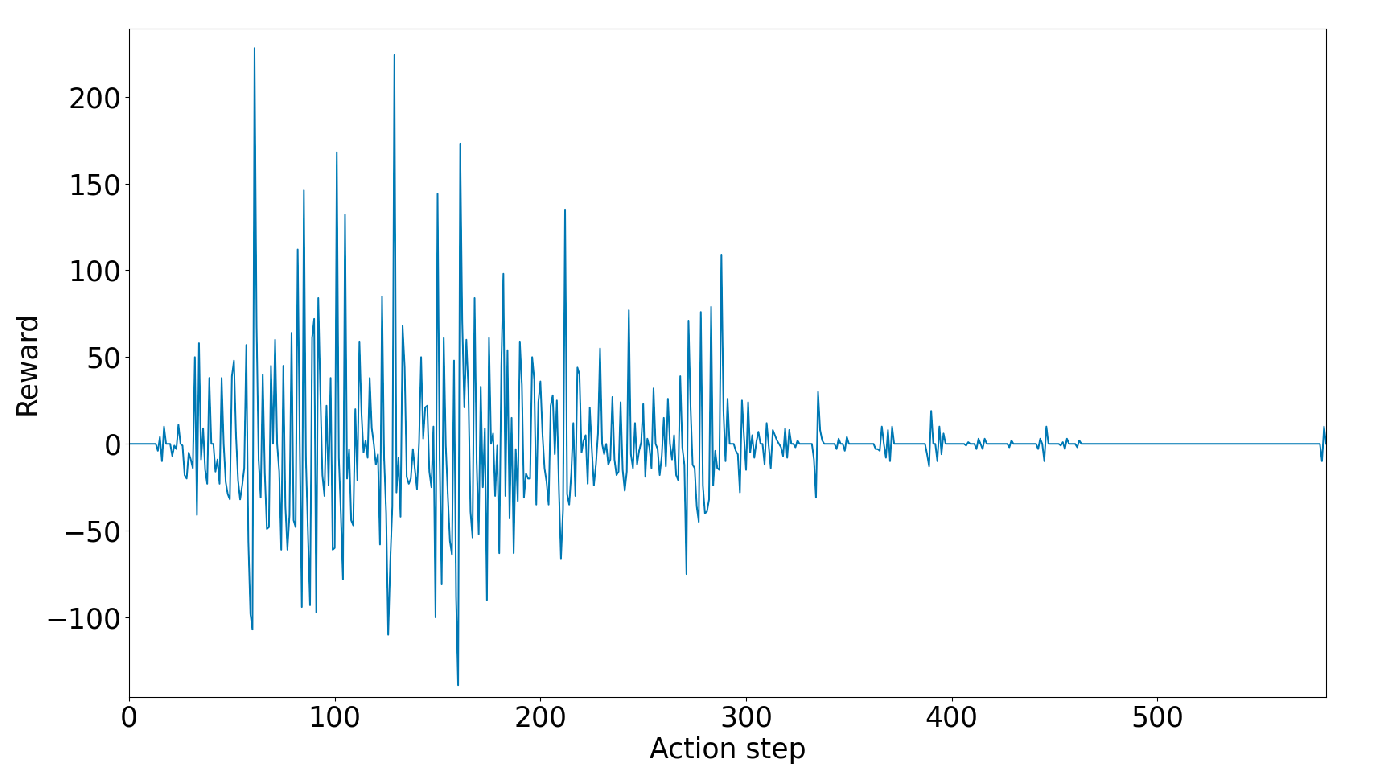
\includegraphics[width=1\linewidth]{images/test_reward.png}
\end{figure}
\end{minipage}
\end{frame}
%%%%%%%%%%%%%%%%%%%%%%%%%%%%%%%%%
%%%%%%%%%%%%%%%%%%%%%%%%%%%%%%%%%
\begin{frame}
\frametitle{Introduction}
\begin{itemize}
  \item  Introduction
  \item Literature Review
  \item System Modeling and Problem Formalization
  \item Deep Q-Learning Algorithm
  \item Simulation Settings
  \item Simulation Results
  \item {\color{cor1}\textbf{Conclusion}}
\end{itemize}

\end{frame}
%%%%%%%%%%%%%%%%%%%%%%%%%%%%%%%%%
%%%%%%%%%%%%%%%%%%%%%%%%%%%%%%%%%
% Slide  (Conclusion)
%%%%%%%%%%%%%%%%%%%%%%%%%%%%%%%%%
% Slide 3 (Conclusion)
\begin{frame}
\frametitle{Conclusion}
\framesubtitle{}
\begin{enumerate}
    \item Experience replay is coupled with the Q- learning to eliminate the correlation in the observation sequence; consequently, improve the model performance.
    \item \textbf{SUMO} environment was generated to train and test the traffic light system (agent).
    \item Two metrics have been employed to evaluate the agent behaviour: 
    \begin{enumerate}
    \item Average queue length (numbers of vehicles)
    \item Accumulative delay time for all vehicles at intersection. 
    \end{enumerate}
    \item The results demonstrated that the proposed algorithm leads to a fair traffic control policy that \textbf{maximize} the \textbf{traffic flow }and \textbf{reduce} the \textbf{accumulative waiting time}.
    \item \textbf{Future work} aims to improve the learning approach to
accelerate convergence and avoid the occurrence of negative
rewards.
\end{enumerate}


\end{frame}

\begin{frame}
\frametitle{Contribution}
\framesubtitle{}
\vspace{1cm}
\begin{minipage}{0.5\textwidth}
\textbf{Walid:}\\
\begin{itemize}
    \item Problem formalization
    \item Environment creation and System Modelling
    \item Deep Q-learning training 
\end{itemize}
\end{minipage}%
\hfill
\begin{minipage}{0.5\textwidth}
\textbf{Siba:}\\
\begin{itemize}
    \item Problem formalization
    \item Environment creation and System Modelling
    \item Deep Q-learning testing 
\end{itemize}
\end{minipage}


\end{frame}
%%%%%%%%%%%%%%%%%%%%%%%%%%%%%%%%%
\end{document}